\label{sec:prespecified}

This audit distinguishes three categories of analysis, and the distinction is load-bearing
throughout the paper: \emph{prespecified} (fixed before the results that would evaluate it were
seen), \emph{post-hoc but qualification-audited} (marker 7, discovered only after seeing
downstream results but subsequently run through the same audit machinery as the prespecified
markers), and \emph{exploratory methodological refinement} (analyses -- most importantly the
nested/refit confounder audit in Section~\ref{sec:confounder-audits} -- introduced after initial
review of the prespecified results, in response to a legitimate methodological concern, and
applied uniformly rather than selectively). We do not claim the entire study was prespecified;
we claim that specific, identifiable components were, and we label the rest explicitly rather
than letting the distinction blur.

\subsection{The six prespecified candidates}

Six candidate markers -- a target and a training cohort each -- were fixed, along with the full
evaluation protocol, before any confounder audit, cross-encoder replication, or downstream
outcome experiment was run (frozen 2026-07-30; internal protocol-freeze record, timestamped
before the LEOPARD, PRECISE, and site-split experiments that would evaluate these criteria):

\begin{enumerate}
\item[(1)] H\&E $\rightarrow$ Gleason score (NADT-Prostate, RidgeCV)
\item[(2)] H\&E $\rightarrow$ phenotype, tumor vs.\ benign (NADT-Prostate, logistic regression)
\item[(3)] ERG-stained image $\rightarrow$ Gleason score (NADT-Prostate, RidgeCV)
\item[(4)] H\&E $\rightarrow$ PTEN copy-number loss (TCGA-PRAD, logistic regression)
\item[(5)] H\&E $\rightarrow$ SPOP mutation (TCGA-PRAD, logistic regression)
\item[(6)] H\&E $\rightarrow$ AR-activity score (TCGA-PRAD, RidgeCV)
\end{enumerate}

Also fixed in advance, before results: the confounders to be controlled for (Gleason grade,
institution/site, scanner, physical tile scale, co-occurring molecular variants, specimen type);
the cross-validation and transfer-evaluation vocabulary (internal CV, zero-shot transfer, native
refit, leave-one-site-out, kept strictly distinct in reporting -- Section~\ref{sec:gates}); one
fixed hyperparameter protocol for every marker and cohort (Section~\ref{sec:gates}); the
multiple-comparison family and minimum-effect-size thresholds for pool membership
(Section~\ref{sec:gates}); the five reliability tiers (Section~\ref{sec:gates}); and the rule
for which markers belong to which of the three LEOPARD evidence pools (naive / qualified /
all-candidate) used in Section~\ref{sec:recurrence-transfer}. Figure~\ref{fig:protocol}
summarizes how a candidate moves from this fixed starting point through the protocol to a tier
assignment.

\begin{figure}[htbp]
\centering
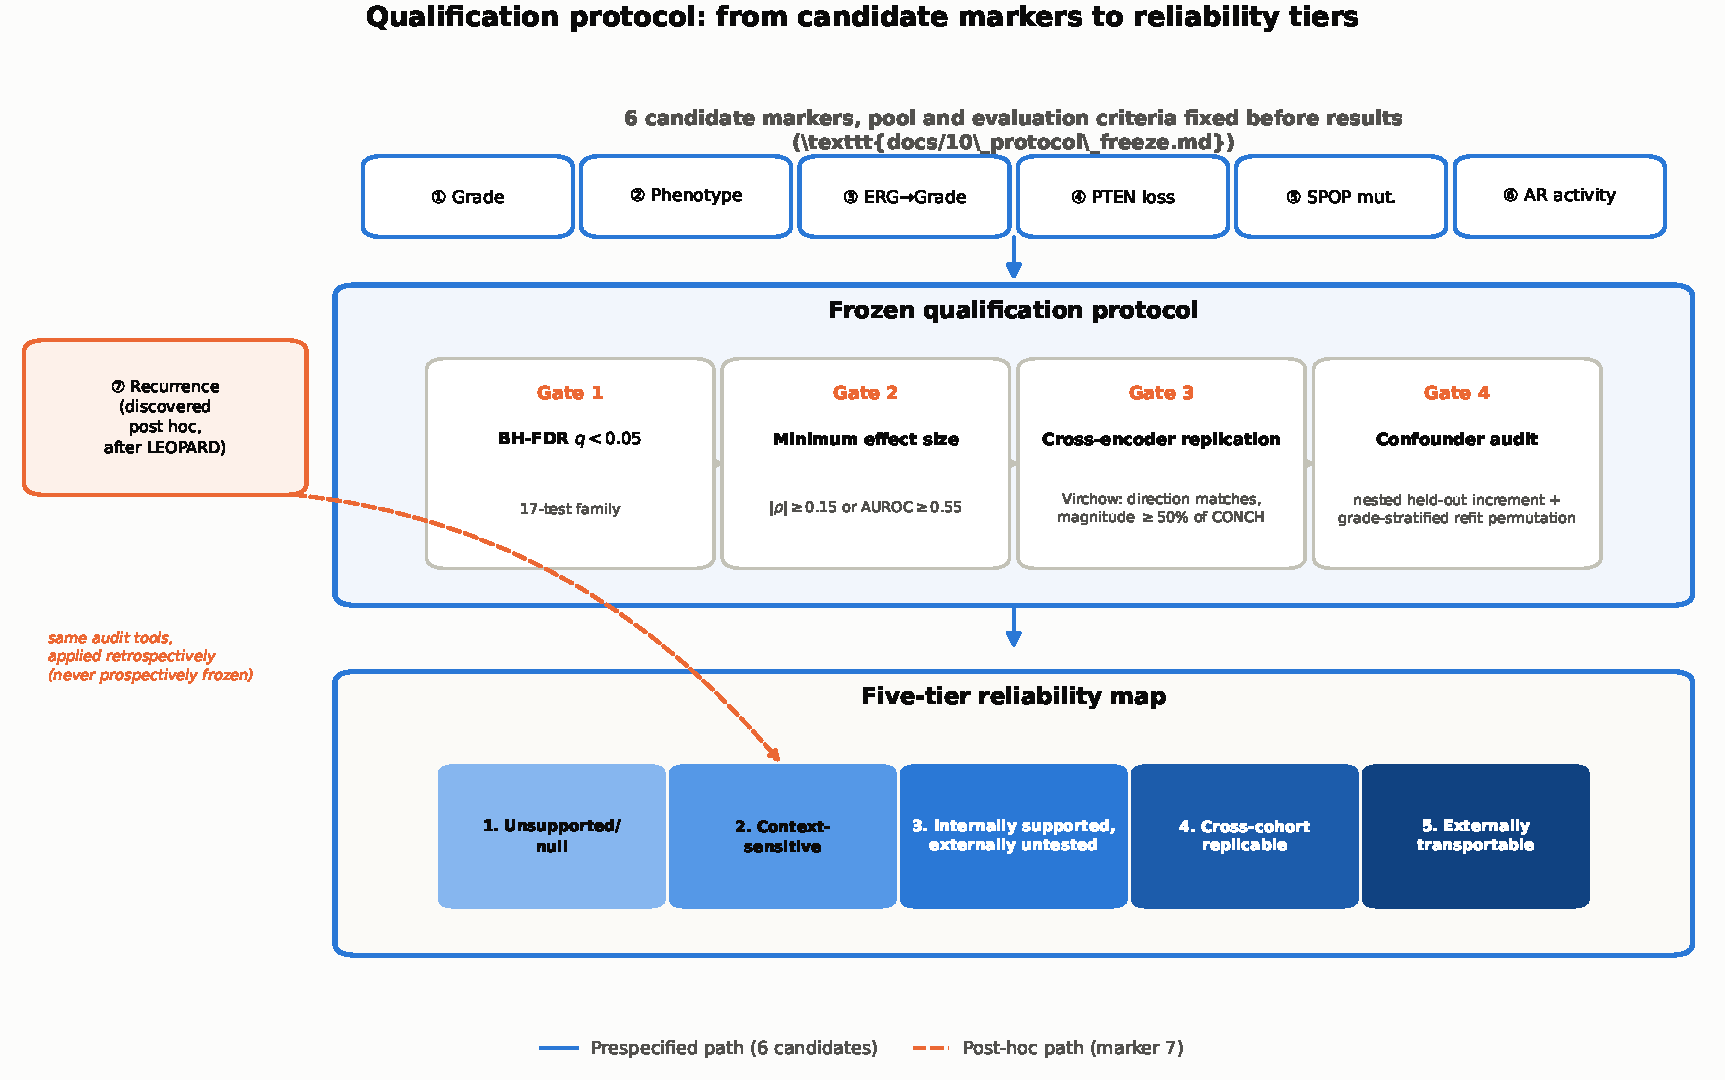
\includegraphics[width=0.95\textwidth]{figures/fig1_protocol_schematic.pdf}
\caption{Qualification protocol: six candidate markers, fixed before results, pass through four
frozen gates to a five-tier reliability assignment. Marker 7 (right) is discovered post hoc and
audited with the same tools, but was never subject to the prospective freeze.}
\label{fig:protocol}
\end{figure}

\subsection{Marker 7: post hoc, audited, never frozen}

A seventh marker -- H\&E $\rightarrow$ biochemical-recurrence risk, fit directly against
recurrence rather than against any of markers 1--6's targets -- was discovered in the course of
running the LEOPARD experiment (Section~\ref{sec:recurrence-transfer}) and was, by construction,
never part of the prospective freeze: its existence depended on having already seen LEOPARD's
recurrence labels. We do not retroactively grant it prospectively-frozen status, and every table
and figure in this paper labels it \emph{post hoc}. What we do provide is the same battery of
qualification tools applied to it retrospectively -- nested confounder audit, grade-stratified
refit permutation, cross-encoder replication, external-endpoint benchmarking -- so that its
evidence is of a comparable rigor to the six frozen candidates even though its discovery process
was not.

\subsection{Exploratory methodological refinement: the nested/refit confounder audit}

The confounder audit design itself has one honest wrinkle worth stating plainly. The originally
frozen design compared clinical-only, image-only, and combined models using image scores that
were already out-of-fold for markers 4 and 6, but computed the incremental-value test
(likelihood-ratio, and a label-permutation test with the image score held fixed) in-sample on
the full cohort -- standard practice for this kind of nested-model comparison, but weaker than a
fully held-out design. In response to external review, we re-ran the same audit with a stricter
nested outer/inner cross-fitting design (the image probe itself refit inside each outer fold,
and refit again inside every permutation) and found the incremental-value conclusions for PTEN
and AR were \emph{not} robust to this stricter test. For marker 7, the completed paired
common-cohort R4 analysis found a positive reconstructed-endpoint grade-level delta C-index,
but its paired IBS and all official-PFI comparison intervals include zero.
We report both versions (Tables~\ref{tab:confounder-4-6} and~\ref{tab:confounder-7}) rather
than only the version that supports a cleaner narrative, and we treat the nested version as
authoritative. This refinement
was introduced after seeing the original results, is not itself prospectively frozen, and is
disclosed as such -- but it was applied uniformly to every marker the original audit covered,
not selectively to the ones expected to survive it.

\subsection{Gate A sensitivity audit and Gate B framing}

The subsequently approved Gate A audit is a descriptive, correlated sensitivity analysis,
not a new confirmatory family. It crosses six markers with CONCH/Virchow, 16/32/64 tiles per
slide, five repeated tile-sampling seeds, and each encoder's native physical scale versus the
shared $1.76\,\mu$m/px scale. Its 360 correlated cells reuse the same frozen cohorts and folds
and are summarized as 72 five-seed configurations and 390 within-design paired contrasts.
The five-seed Student-$t$ intervals quantify variation across repeated tile sampling on those
same data; they are not patient-level or population confidence intervals. The approved Gate B
framing is that Gate A did not overturn the prior directional observations. Instead, it bounds
generalizability across configuration, endpoint, encoder, and site; where evidence is
insufficient, the claim remains unresolved rather than contrary evidence. C04 and C05 retain
their approved uncertainty after completed R5 evidence closure. C06 has completed the
common-498 R2 and official-PFI R3 sensitivities; C07 is closed narrowly by the completed paired
common-cohort R4 analysis. No grid setting was selected, recalibrated, or
relabeled after observing its result.
